\EXERCISE
فردی قصد دارد تا از نقطه‌ی $A$ به نقطه‌ی $C$ برود، اما با این شرط که:
\begin{itemize}
    \item 
   در هر حرکت روی یک ضلع شبکه حرکت کند.

    \item 
 هر حرکت به سمت بالا یا راست باشد.
 
	\item 
از نقطه ی $B$ عبور نکند.
\end{itemize}

حال او به چند روش میتواند از $A$ به $C$ برود؟

    \begin{center}
     	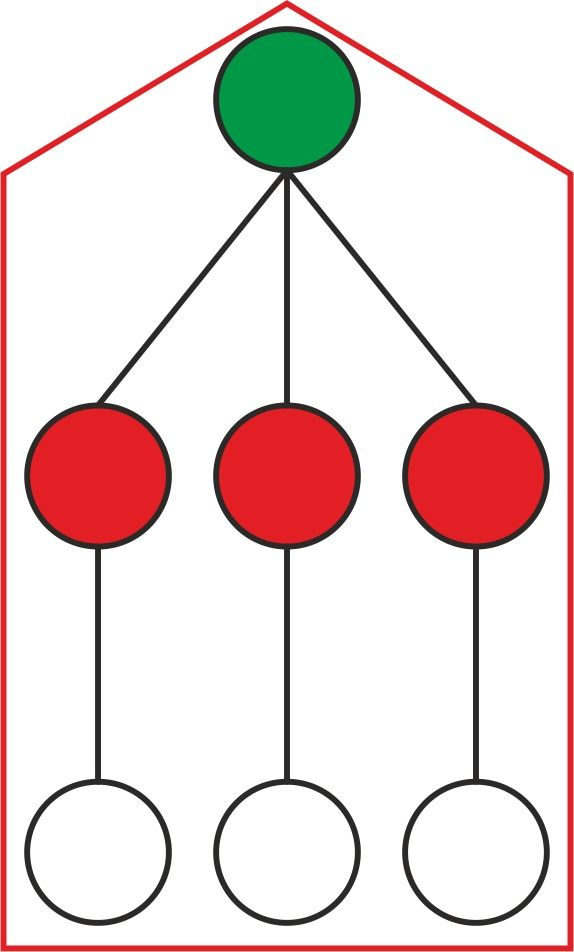
\includegraphics[scale=0.2]{./6.png}
    \end{center}